\subsection{Datasets}
\subsubsection{DBLP dataset and other citation networks}
\subsubsection*{Description of Dataset}
DBLP is a online publication database, focused on Computer Science. 

A labelled subset of DBLP is used in our experiment. It consists of 14,376 papers, 14,475 authors, 8920 terms, 20 conferences in total. A fraction of nodes are labelled with which of the following four fields it belongs to, AI, DM,IR and DB. Among the labelled nodes, 4057 authors, 100 paper, 20 conference are included.
\subsubsection*{Graph Construction and Information}
The graph is constructed as follows: we simply put all the nodes together. So it will be heterogeneous. The basic information about this graph is shown in the Table 1 and 2.

\begin{table}[!ht]
\centering
\begin{tabular}{cc}
\toprule
\textbf{\#nodes} & \textbf{\#edges}\\
\midrule
4177 & 170794\\
\bottomrule
\end{tabular}
\caption{DBLP Network}
\end{table}

\begin{table}[!ht]
\centering
\begin{tabular}{cccc}
\toprule
\textbf{\#DB} & \textbf{\#DM} & \textbf{\#AI} & \textbf{\#IR}\\
\midrule
1230 & 763 & 1029 & 1155\\
\bottomrule
\end{tabular}
\caption{Distribution of labels in DBLP Network}
\end{table}

The network is illustrated in Figure 3.

\begin{figure}[!ht]
	\centering
	\begin{minipage}[b]{0.5\linewidth}
	\centering
	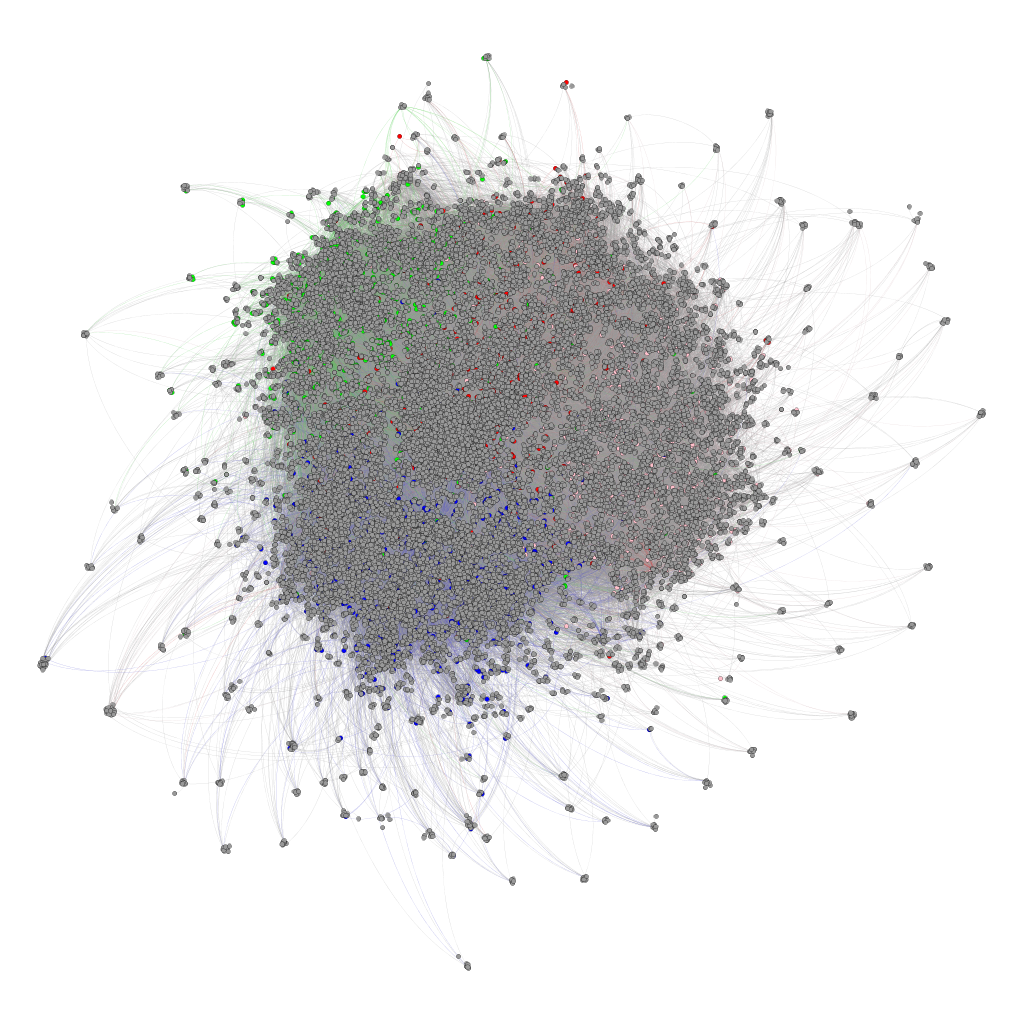
\includegraphics[width=\textwidth]{FIG/dblp.png}
	\caption{Visualization of DBLP network}
	\label{fig:figure1}
	\end{minipage}
\end{figure}	

\subsubsection{Social Networking(KDD Cup 2012)}

\subsubsection*{Description of Dataset}
This dataset comes from Tencent Weibo, one of the largest micro-blogging website in China.
It contains many different types of information and was chosen to be the material for KDD Cup 2012.

Despite the original purpose of the competition of KDD Cup, we found something interesting from the dataset:
We can get the label of some users. There is a category system in which users are labeled with hierarchy categories. And there is a following history for each user.

\subsubsection*{Graph Construction and Information}
As the BP algorithm is defined on undirected graphs, we need to fit the dataset into a more applicable format.
The following relationship is naturally uni-directional, however, most people would follow back to his/her follower if he/she found that the particular follower is similar to himself/herself.
Thus, we can keep the users and their bi-directional relationship to get a undirected graph in which edges indicates the similarity of two nodes.

After filtering the dataset, we extracted all users labeled ``1.1", ``1.4" or ``1.6", constructing a graph with 1741 nodes and 18718 edges.


\subsubsection{Amazon Product co-purchasing networks}

\subsubsection*{Description of Dataset}
This network represents co-purchasing relationship between products on Amazon website. Most nodes fell into four major categories: Book, Music, DVD and Videos. The whole net work consists of 542684 nodes and 3387388 edges in all.


\subsubsection*{Graph Construction and Information}
Although the relationship of this network is defined as co-purchasing, actually it is not symmetry. So we first filter a subgraph, in which each edge represents mutual co-purchasing relationship. The basic information of this mutual co-purchasing network is illustrated in Table 3 and 4. 

Because this a huge graph, the full scale picture of this graph mixed everything together and it is hard to tell any useful pattern from this graph, so we randomly sample a 5000 node subgraph, which is shown Figure 5.

\begin{table}[!ht]
\centering
\begin{tabular}{cc}
\toprule
\textbf{\#nodes} & \textbf{\#edges}\\
\midrule
393361 & 922867\\
\bottomrule
\end{tabular}
\caption{Amazon mutual co-purchasing Network}
\end{table}

\begin{table}[!ht]
\centering
\begin{tabular}{cccc}
\toprule
\textbf{\#Books} & \textbf{\#Music} & \textbf{\#DVD} & \textbf{\#Video}\\
\midrule
287678 & 74867 & 18923 & 11893\\
\bottomrule
\end{tabular}
\caption{Distribution of labels in Amazon Network}
\end{table} 

\begin{figure}[!ht]
	\centering
	\begin{minipage}[b]{0.5\linewidth}
	\centering
	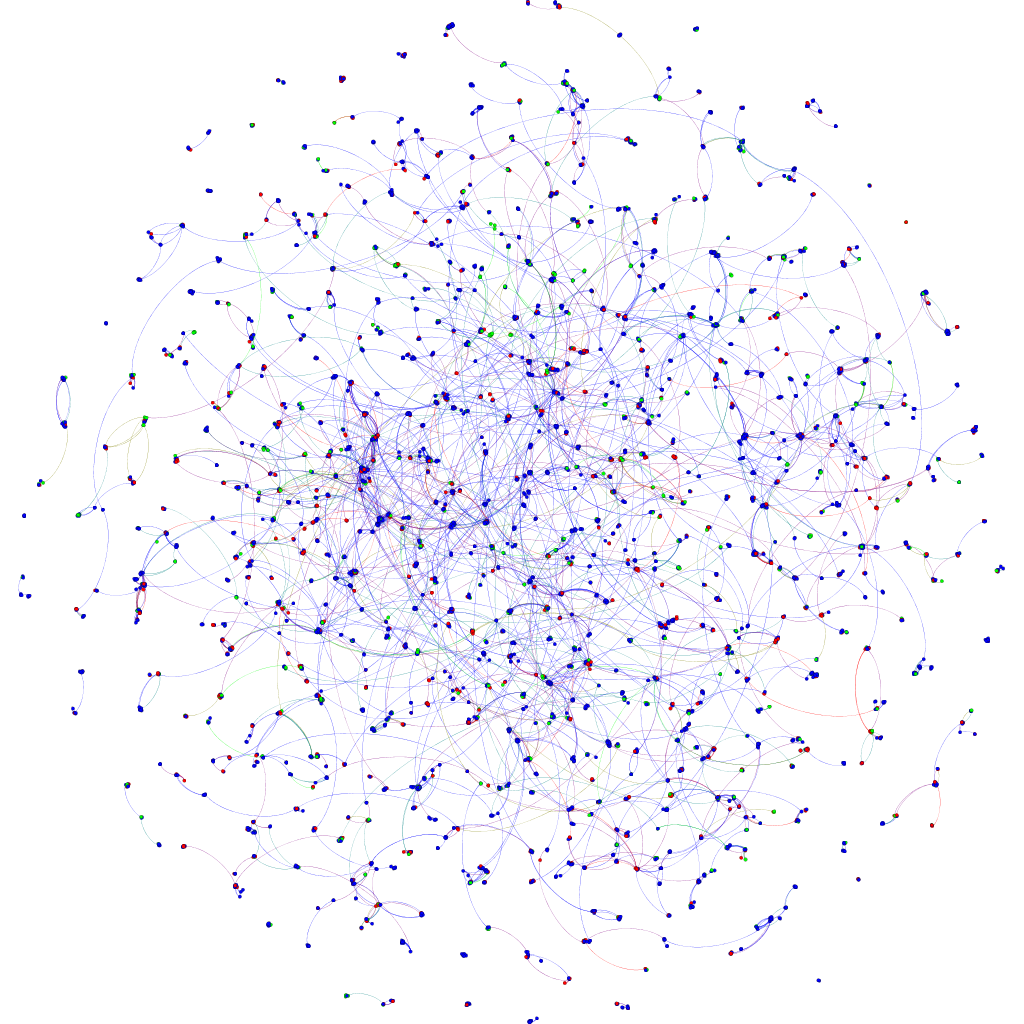
\includegraphics[width=\textwidth]{FIG/amazon.png}
	\caption{Visualization of Amazon network}
	\label{fig:figure1}
	\end{minipage}
\end{figure}	


\subsubsection{Flickr photo network}

\subsubsection*{Description of Dataset}
This data set is from MIR (Multimedia Information Retrieval) FLICKR Retrieval Evaluation.In this dataset, photos are associated with one or more tags from Flickr user. Photos are also annotated manually by annotator with a category. We build this network of photos based on whether two photos share same tags. 

There are 22,872 photos that have at least one tag in this dataset. Tags are from Flickr users, like ‘dog’, ‘doors’, ‘ocean’ etc. For photos with at least one tag, each of them is associated with 9.8 tags on average. The photo with largest number of tags has 75 tags. The photo with smallest number of tags has only 1 tag. The number of photos only with 1 tag is 813. The number of photos with 2 tags is 987.

The photos are manually annotated with one or more of the 24 categories like ‘animals’, ‘baby’, ‘indoor’ etc. There are 24,581 photos with at least one category. For photos with at least one category, each of them is associated with 3.8 categories on average.  The most widely used category is ‘people’ (10,373 times) followed by ‘structures’ (9992 times). 

\subsubsection*{Methods of Experiments on Dataset}
We can build a network of photos based on whether two photos share tags. If we build a network of photos based on whether two photos share 1 tag, the average degree is 781. If we build a network of photos based on whether 2 photos share at least two tags, the average degree is 92. If we build a network of photos based on whether two photos share at least 3 tags, the average degree is 16. In later experiment, we can try different network building criterion.

With this network of photos, we can run BP and \textbf{FaBP}, and predict the category of photos.


\subsection{Experiment Settings}
\subsubsection*{Overview}
In order to validate the performance of our proposed methods, on each graph we carried out the following experiments:
\begin{enumerate}
	\item \textbf{MBP}: Multiclass BP
	\item \textbf{OVA}: One-VS-ALL schema using \textbf{FaBP} as underlying classifier
	%\item \textbf{AVA}: All-VS-All schema using \textbf{FaBP} as underlying classifier
	\item \textbf{ECOC}: Error correcting code schema using \textbf{FaBP} as underlying classifier
\end{enumerate}

\subsubsection*{Multiclass BP}
In order to run Multiclass BP, we should first speicfy the following parameters:
\begin{itemize}
	\item \textbf{$\phi$} : Priors for all the nodes.
	\item \textbf{$\psi$} : The correlation matrix which specifies the \textit{closeness} between two of labels. 
\end{itemize}

To estimate $\pi$, before each experiment, we randomly select $p\%$ of the set of nodes whose labels are already known to us. The $p\%$ for each graph is listed in Table ?.

\begin{table}[!ht]
\centering
\begin{tabular}{c|c}
\toprule
\textbf{Datasets} & \textbf{p}\\
\midrule
DBLP & 20\%\\
Flickr & 8\%\\
Tencent & 5\%\\
Amazon & 30\%\\
\bottomrule
\end{tabular}
\caption{Percentage of labelled data in prior $\phi$}
\end{table} 

As to correlation matrix $\phi$, we estimate this matrix using the following strategy: for a pair of given labels, say A and B, we calculate all the edges between the two labels, denoted as $\#(AB)$. For each label, we also compute the number of edges associated with that label, which means all the edges that have at least one end being the given label. In our case, we denote them as $\#(A)$ and $\#(B)$. Then $\psi$ is defined as follows:
\begin{gather*}
	\psi_{A\rightarrow B} = \frac{\#(AB)}{\#(A)}\\
	\psi_{B\rightarrow A} = \frac{\#(AB)}{\#(B)}
\end{gather*}

Repeat the above procedure for each pair of labels, then we have the estimation of the correlation matrix.

\subsubsection*{One-VS-All with \textbf{FaBP}}
\textbf{FaBP} algorithm is parameterized by one single important factor: the "about-half" homophily factor, denoted as $h_h$. The bigger $h_h$ means the stronger the homophily phenomenon in the graph.

\begin{table}[!ht]
\centering
\begin{tabular}{c|c}
\toprule
\textbf{Datasets} & \textbf{$h_h$}\\
\midrule
DBLP & 0.002\\
Flickr & 0.2\\
Tencent & 0.002\\
Amazon & 0.01\\
\bottomrule
\end{tabular}
\caption{The homophily factor for each network}
\end{table} 

As to the prior $\phi$, we follows the same settings with \textbf{MBP}.

When the algorithm finished, for each node, say $N$, we combine all the k probabilities $P(N=k_i)$ in a vector, which specifies how likely the given node is within that class. Then we pick the class that has the greatest $P(N=k_i)$ as the label of that node.

\subsubsection*{ECOC with \textbf{FaBP}}
The settings of prior $\phi$ and homophily factor $h_h$ is the same as those in \textbf{OVS}.

When coming to the code design, we adopts the exhaustive algorithm described in \cite{Thomas1995}. When given $k$ labels, each label is encoded using $2^{k-1}-1$ bits. For the first class, we encode it using all ones. For the second class, we set the first $2^{k-2}$ bits of its coding as zeros, then the next $2^{k-2}-1$ bits as ones. For the third class, we set the first $2^{k-3}$ bits as zeros, the following $2^{k-3}$ as ones, which are followed by $2^{k-3}-1$ zeros. Repeating the this procedure until all the classes are defined. 

The code matrix when $k=4$ is illustrated in Table 7.

\begin{table}[!ht]
\centering
\begin{tabular}{c|ccccccc}
\toprule
\textbf{class} & 1 & 2 & 3 & 4 & 5 & 6 & 7\\
\midrule
1 & 1 & 1 & 1 & 1 & 1 & 1 & 1\\
2 & 0 & 0 & 0 & 0 & 1 & 1 & 1\\
3 & 0 & 0 & 1 & 1 & 0 & 0 & 1\\
4 & 0 & 1 & 0 & 1 & 0 & 1 & 0\\
\bottomrule
\end{tabular}
\caption{Code design when $k=4$}
\end{table}

As described in \textbf{Methods} section, we run \textbf{FaBP} for each bit. For each node, after we get the probability vector, we transform it into a binary vector, using the following strategy: for a given bit $b_i$, if $P(b_i=1) > 0.5$, then the corresponding position of the binary vector is set to 1, else to zero. Then we calculated the Hamming distance between this vector and coding vector of each class, the one has the smallest distance is assigned to the node. 

\subsection{Experiment Results}
All the results are illustrated in the following table.
\begin{table}[!ht]
\centering
\begin{tabular}{c|ccc}
\toprule
\textbf{Datasets} & \textbf{MBP} & \textbf{OVS} & \textbf{ECOC}\\
\midrule
DBLP &0.17 &\textbf{0.776} &0.726\\
Flickr & \textbf{0.653} & 0.421 & 0.13\\
Tencent & 0.953 & \textbf{0.961} & 0.924\\
Amazon & \textbf{0.736} & 0.636 & 0.626\\
\bottomrule
\end{tabular}
\caption{The homophily factor for each network}
\end{table} 











